\documentclass{beamer}

\mode<presentation> {
	\usetheme{Madrid}
}

\usepackage{graphicx}
\usepackage{booktabs}
\usepackage{cite}
\usepackage{tabularx}
\usepackage{csquotes}
\usepackage{subfig}
\usepackage{media9}

\graphicspath{{images/}}

\title[Robotics \& Automation]{Vision Based Robot Manipulation Testbed for Reinforcement Learning}

\author[CET]{
	Department for Interdisciplinary Research\\ College of Engineering Trivandrum
}

\begin{document}
	
	\begin{frame}
		\maketitle
		
		\begin{tabularx}{\textwidth}{lXl}
			\textbf{Guided by,} & & \textbf{Presented by,} \\
			Linu Shine & & Sreejith Krishnan R \\
			Electronics and Comm. Engg. & & Robotics \& Automation
		\end{tabularx}
	\end{frame}

	\begin{frame}
		\frametitle{Motivation}
		
		\begin{columns}[c]
			\column{0.45 \textwidth}
			Why robot manipulation?
			\begin{itemize}
				\item Assist humans in general tasks
				\item Build machines that can grasp and manipulate objects with human levels of dexterity
			\end{itemize}
			
			\column{0.5 \textwidth}
			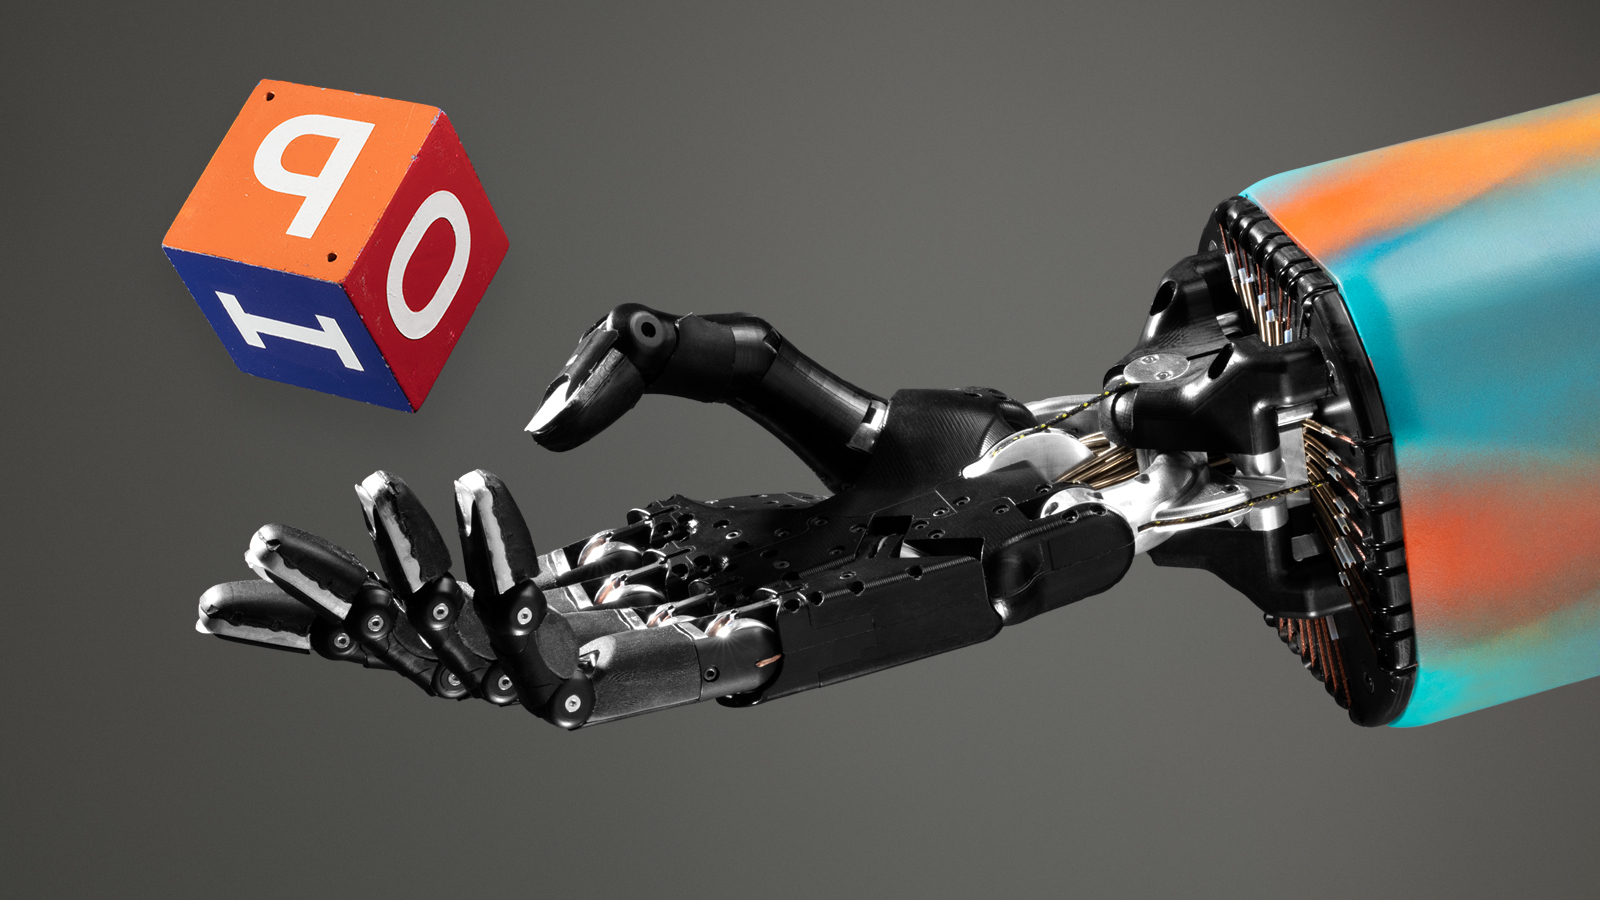
\includegraphics[width=6cm]{learning-dexterity}
		\end{columns}
		
		
		\vspace{2em}
		A reinforcement learning testbed provides,
		
		\begin{itemize}
			\item A standardized benchmarking environment for comparing performance of different RL algorithms
			\item An entry point for quickly testing RL algorithms for robot manipulation tasks enabling quick development
			\item A high performance framework for efficient training of RL algorithms
		\end{itemize}
	\end{frame}
	
	\begin{frame}[allowframebreaks]
		\frametitle{Literature survey}
		
		\begin{tabular}{m{2.25cm} | m{9cm}}
			\hline
			
			\textbf{Title} &
			SURREAL: Open-Source Reinforcement Learning Framework and Robot Manipulation Benchmark \cite{corl2018surreal} - Conference on Robot Learning - 2018\\
			\hline
			
			\textbf{Methodology} &
			\begin{itemize}
				\item Open-source framework for benchmarking reinforcement learning algorithms
				\item Decomposed architecture
				
			\end{itemize}\\
			\hline
			
			\textbf{Merits} &
			\begin{itemize}
				\item Allows scaling RL speed with computation power
				\item Prebuilt standardized environments for common robot manipulation tasks
			\end{itemize} \\
			\hline
			
			\textbf{Demerits} &
			\begin{itemize}
				\item No integration with RayLib - A common framework for scalable reinforcement learning
				\item No prebuilt support for experiment logging and tracking
			\end{itemize}\\
			\hline
			
		\end{tabular}
	
		\begin{tabular}{m{2.25cm} | m{9cm}}
			\hline
			
			\textbf{Title} &
			Comparing Task Simplifications to Learn Closed-Loop Object Picking Using Deep Reinforcement Learning \cite{tasksimplification} - IEEE Robotics and Automation Letters - 2019\\
			\hline
			
			\textbf{Methodology} &
			\begin{itemize}
				\item Uses autoencoder to encode high dimensional camera data to low dimensional encoding
				\item Feed forward neural network predicts action from encoded data
				\item RL to train neural networks
			\end{itemize}\\
			\hline
			
			\textbf{Merits} &
			\begin{itemize}
				\item No hand labeled data required
			\end{itemize} \\
			\hline
			
			\textbf{Demerits} &
			\begin{itemize}
				\item Low success rate (78\%) for manipulation of objects in clutter by real robot
				\item Non modular. Difficult to reuse model for similar task
			\end{itemize}\\
			\hline
			
		\end{tabular}
	
		\begin{tabular}{m{2.25cm} | m{9cm}}
			\hline
			
			\textbf{Title} &
			Regularized Hierarchical Policies for Compositional Transfer in Robotics \cite{rhpo} - DeepMind - 2019\\
			\hline
			
			\textbf{Methodology} &
			Use hierarchical modular policies for continuous control. \\
			\hline
			
			\textbf{Merits} &
			\begin{itemize}
				\item Best sample efficiency on both simulated and real robot
				\item Uses MPO optimization algorithm which reduces the number of hyperparameters
			\end{itemize} \\
			\hline
			
			\textbf{Demerits} &
			\begin{itemize}
				\item High level tasks are not automatically decomposed to sub tasks
				\item Low level policy is shared across all low level tasks making interpretability complicated
				\item Transferring specific skills from sub-tasks policy in a predictable manner is difficult
				\item Experiment results are obtained using model whose inputs include pose of objects in workspace
			\end{itemize}\\
			\hline
			
		\end{tabular}
	\end{frame}
	
	\begin{frame}
		\frametitle{Research Gap and Objectives}
		\textbf{Research Gap}
		\begin{itemize}
			\item Slow training data collection speed
			\item Non standard/readily available frameworks used
		\end{itemize}
		\vspace{1em}
		\textbf{Objective} \\
		\begin{itemize}
			\item Improve RL model training speed by running multiple simulations in parallel
			\item Use standard frameworks that support training distributed RL algorithms
			\item Prebuilt experiment logging and tracking
			\item Flexibility for adding different types of robot manipulation tasks like grasping, moving etc.
		\end{itemize}
	\end{frame}

	\begin{frame}[allowframebreaks]
		\frametitle{Methodology}
		
		\begin{columns}[c]
			\column{0.45 \textwidth}
			\begin{itemize}
				\item Simulation environment created on Bullet Physics Simulator
				\item Experiments will be run in distributed fashion
				\item Simulator tuned for maximum throughput
				\item Integrated with RayLib for scaling reinforcement learning
				\item Experiment logging, tracking and visualization using comet.ml platform
				\item Easy to add new robot manipulation tasks
			\end{itemize}
			
			\column{0.5 \textwidth}
			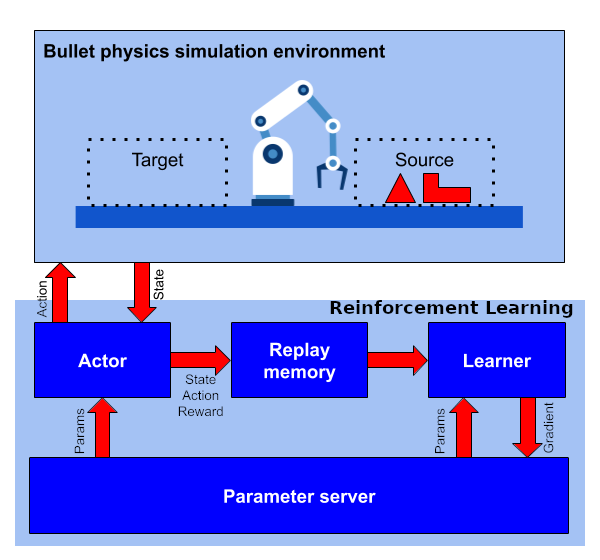
\includegraphics[width=6cm]{setup}
		\end{columns}
	
		\begin{columns}[c]
			\column{0.5 \textwidth}
			\begin{itemize}
				\item Simulated robot tuned to have properties similar to real ABB IRB 120 robot
				\item Graphics rendering can be disabled to speedup simulator
				\item Grasp detection and collision detection algorithms for easy reward calculation
				\item Multiple simulator instances can be run parallel
			\end{itemize}
			
			\column{0.5 \textwidth}
			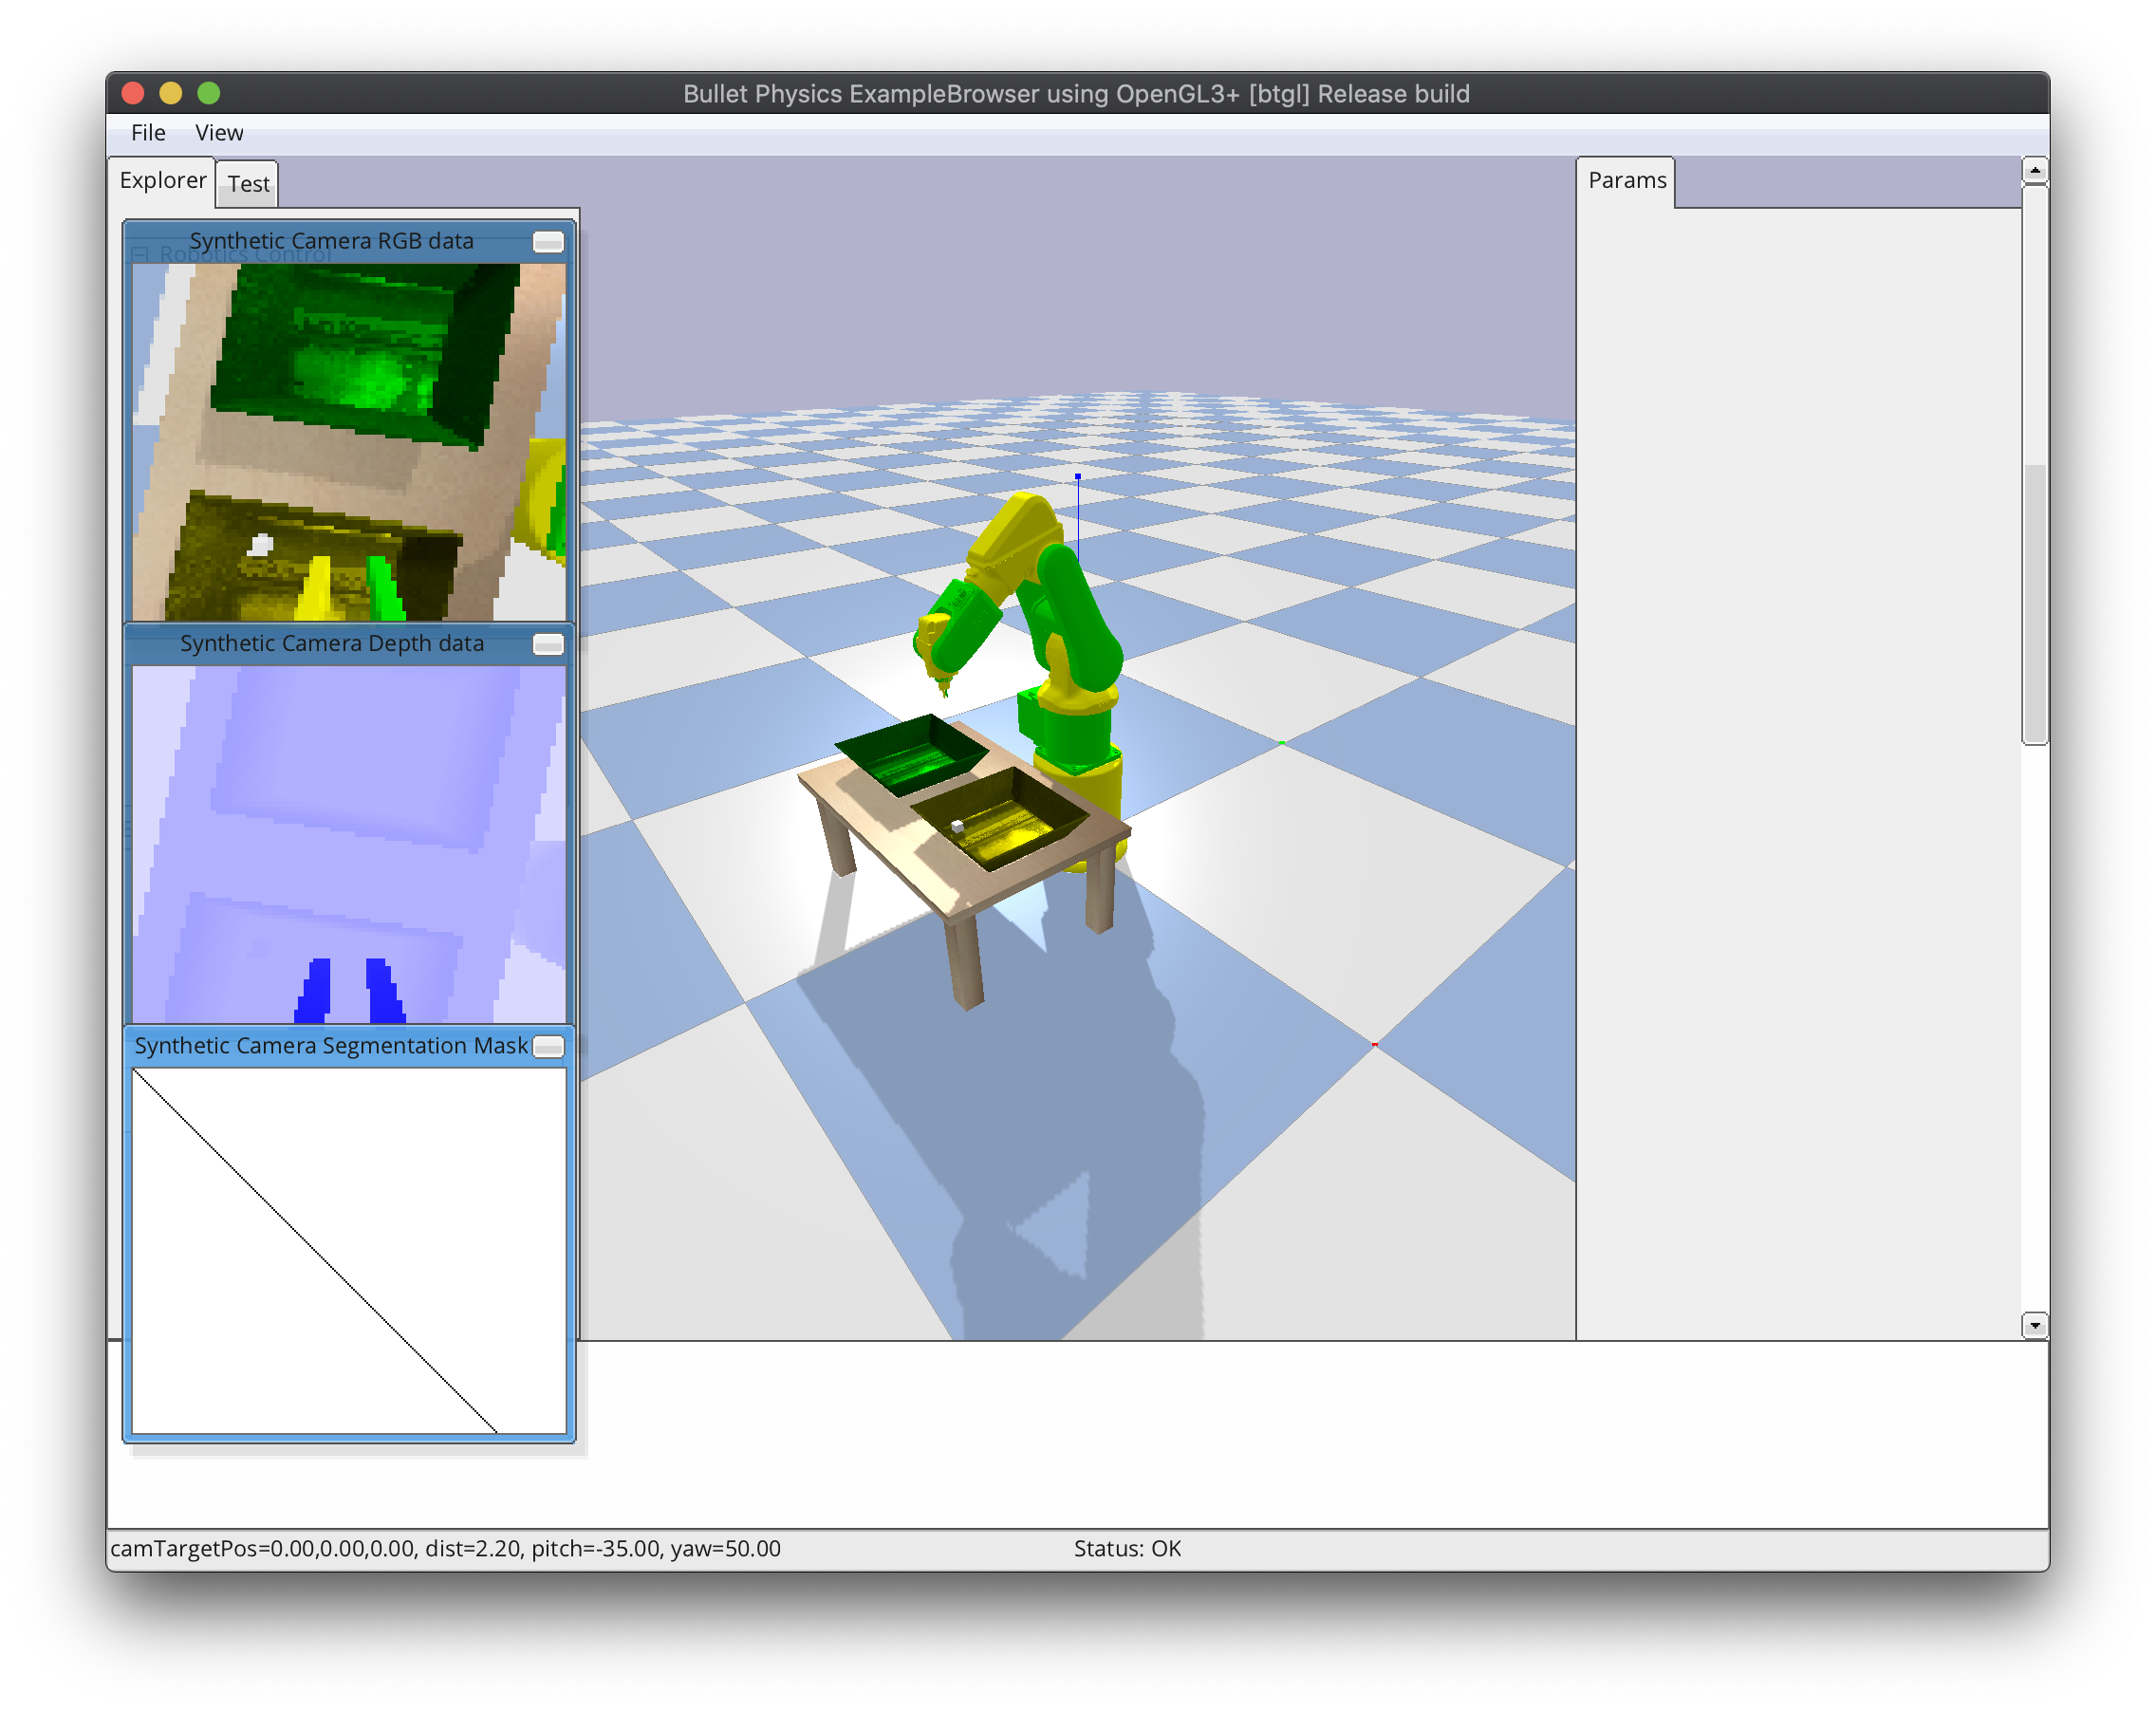
\includegraphics[width=6cm]{simulator.png}
		\end{columns}
	\end{frame}

	\begin{frame}
		\frametitle{Experiment Setup}
		
		\begin{columns}[c]
			\column{0.5 \textwidth}
			\begin{itemize}
				\item Task is to move the object from yellow tray to green tray
				\item RGB-D camera is mouted on end effector
				\item Input to RL model is depth image from RGB-D camera
				\item Observation space is of shape $84x84x4$
				\item Action space is $[\delta x, \delta y, \delta z, \delta r_x, open]$ which can be used for relative movement and rotation of end effector 
			\end{itemize}
			
			\column{0.5 \textwidth}
			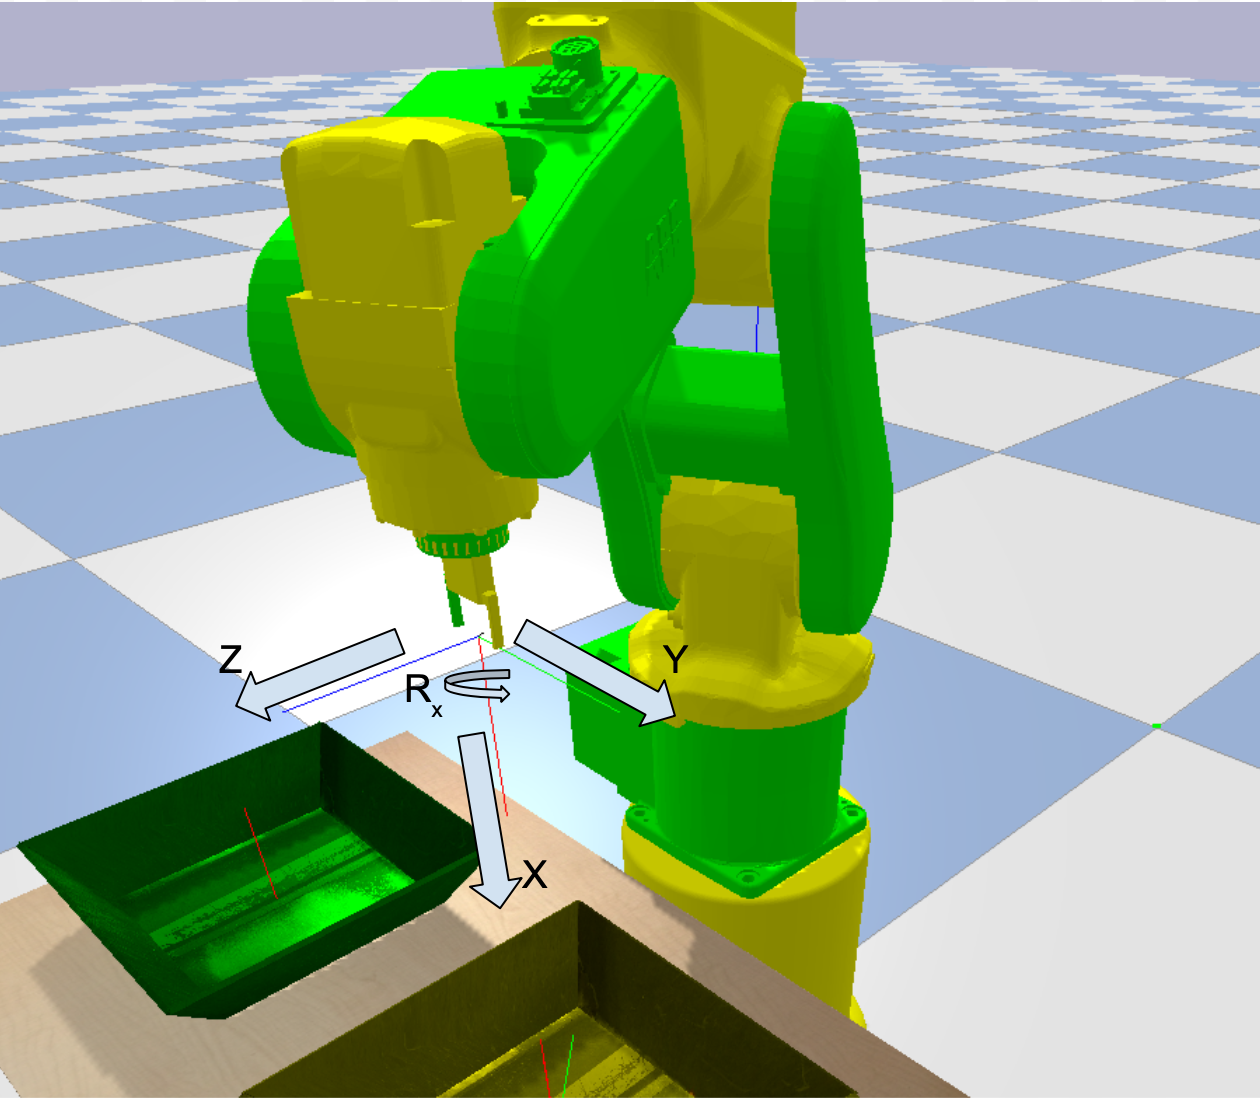
\includegraphics[width=6cm]{action-space.png}
		\end{columns}
	\end{frame}

	\section{Results}
	\begin{frame}
		\frametitle{Results}
		\framesubtitle{Simulator performance}
		
		\begin{columns}[c]
			\column{0.5 \textwidth}
			\begin{itemize}
				\item Mean action time of 0.053 seconds without rendering and 0.345 seconds with rendering
				\item 2.4 times faster than data collection from real robot when rendering is enabled
				\item 17.2 times faster than data collection from real robot when rendering is disabled
			\end{itemize}
			
			\column{0.5 \textwidth}
			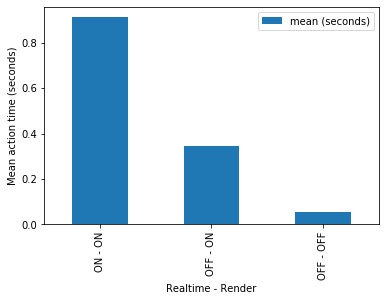
\includegraphics[width=6cm]{benchmark-table-clearing.png}
		\end{columns}
	
	\begin{table}
		\begin{tabular}{|c|c|c|c|c|c|}
			\hline
			\textbf{Render | Realtime} & \textbf{Mean} & \textbf{Std} & \textbf{25\%} & \textbf{50\%} & \textbf{75\%} \\
			\hline
			ON | ON & 0.912 & 2.783 & 0.358 & 0.374 & 0.39 \\
			\hline
			ON | OFF & 0.345 & 0.583 & 0.198 & 0.206 & 0.214 \\
			\hline
			OFF | OFF & 0.053 & 0.023 & 0.046 & 0.047 & 0.048 \\
			\hline
		\end{tabular}
	\end{table}
	\end{frame}

	\begin{frame}
		\frametitle{Results}
		\framesubtitle{Baseline PPO}
		\begin{columns}[c]
			\column{0.6 \textwidth}
			\begin{itemize}
				\item Convolution layers are used for feature extraction
				\item Input in RGB-D 84x84x4 matrix
				\item Value network predicts the how good it is to be at a particular state
				\item Policy network directly predicts the mean and standard deviation of a Gaussian PDF from which actions are sampled for a particular state
				\item Train batch size is 10240 and SGD minibatch size is 512. Number of iterations per train batch is 30
				\item Data from an episode is added to train batch only after the it is complete
			\end{itemize}
			
			\column{0.4 \textwidth}
			\begin{figure}
				\small{Architecture}
				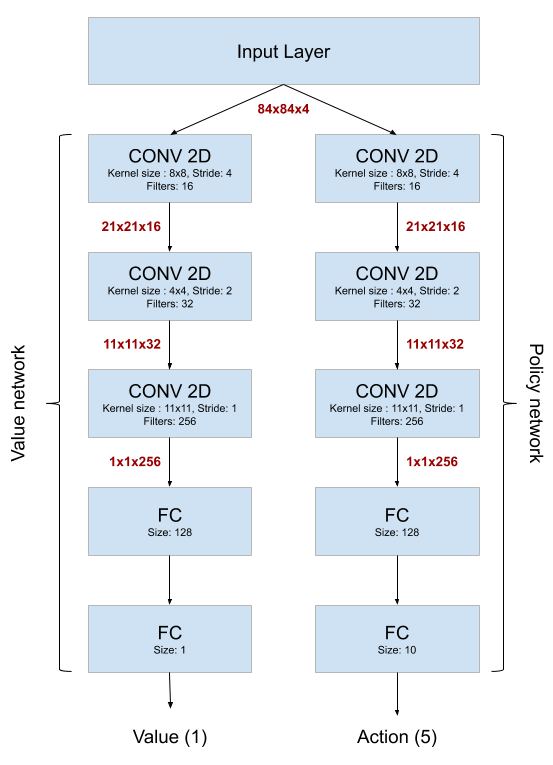
\includegraphics[scale=0.25]{visionnet-arch.png}
			\end{figure}
		\end{columns}
	\end{frame}

	\begin{frame}
		\frametitle{Results}
		\framesubtitle{Baseline PPO}
		\vspace{-2em}
		\begin{columns}[c]
			\column{0.5 \textwidth}
			\begin{itemize}
				\item Model learns to avoid collision after training for 4M timesteps
				\item Optimum reward values for grasping and drop penalty is not reached after training for 4M timesteps
				\item From other research papers, PPO network needs to be trained for approximately
				80M timesteps to reach optimum reward values
			\end{itemize}
			
			\column{0.45 \textwidth}
			\begin{figure}
				\begin{tabular}{c}
					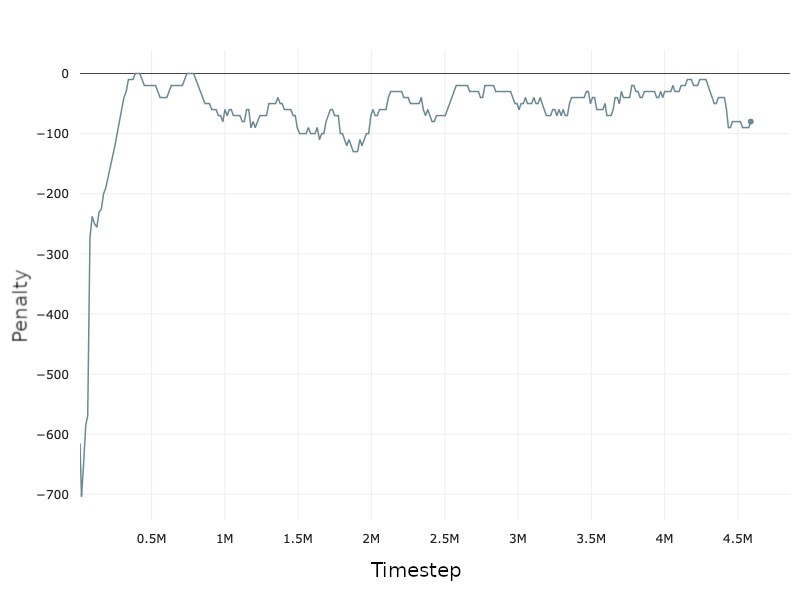
\includegraphics[scale=0.65]{ppo-simulation-collision-penalty.jpeg} \\
					{\small Collision penalty. Optimum value is 0} \\ 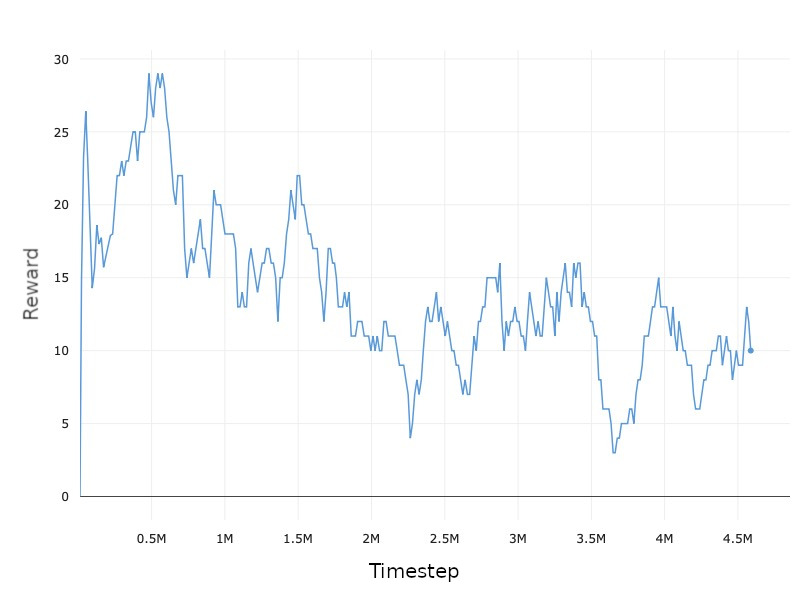
\includegraphics[scale=0.65]{ppo-simulation-grasp-reward.jpeg} \\
					{\small Grasp reward. Optimum value is 100} \\
				\end{tabular}
			\end{figure}
		\end{columns}
	\end{frame}

	\begin{frame}
		\frametitle{Results}
		\framesubtitle{Baseline PPO}
		\vspace{-1em}
		\begin{columns}[c]
			\column{0.5 \textwidth}
			\begin{itemize}
				\item Reward shaping is critical. Small changes in reward function can change the learning process.
				\item Providing +ve reward when end effector moves towards target and -ve reward when end effector moves away will not work
				\item Initializing each episode at a random state like grasped and not grasped can improve training speed
			\end{itemize}
			
			\column{0.5 \textwidth}
			\begin{figure}
				\begin{tabular}{c}
					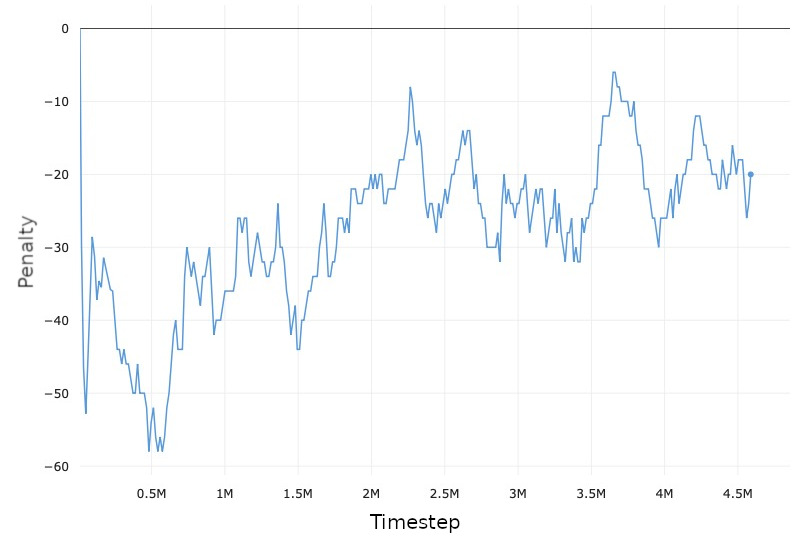
\includegraphics[scale=0.65]{ppo-simulation-drop-penalty.jpeg} \\
					{\small Drop penalty. Optimum value is 0} \\ 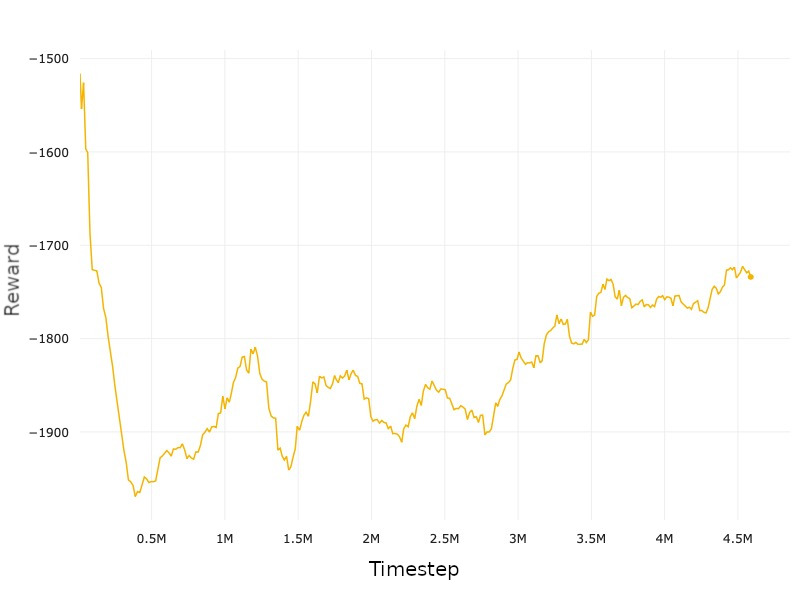
\includegraphics[scale=0.65]{ppo-simulation-reward-mean.jpeg} \\
					{\small Mean reward. Optimum value $>$ 200} \\
				\end{tabular}
			\end{figure}
		\end{columns}
	\end{frame}

	\section{Future scope}
	\begin{frame}
		\frametitle{Future scope}
		
		\begin{itemize}
			\item Including DDPG and RHPO baseline models
			\item Evaluating baseline models on real robot
			\item Including more common robot manipulation tasks to testbed
			\item Including baseline support for multi agent robot manipulation tasks
		\end{itemize}
	\end{frame}

	\begin{frame}[allowframebreaks]
		\frametitle{Challenges}
		
		\begin{itemize}
			\item Initially objective of this project was to evaluate Regularized Hierarchical Policy Optimization (RHPO) for robot manipulation tasks
			\item To train RHPO for table clearing task, computations must be run on machine with 32 CPU cores and NVIDIA V100 GPU for approx 2 days
			\item In CET, computer cluster with more than 32 CPU cores is available. But it does not have GPU. Efforts were made to try and use compute cluster from CET for running simulations and use GPU from google colab for training neural networks, but slow networking speed made the training process extremely slow
			\item Also efforts were made to use both GPU and CPU from google cloud by using 300 USD trial provided by google cloud. But restrictions in running time of preemptible virtual machines prevented this strategy
			\item Hence the objective of the project was changed to development of testbed which require lower compute power since only simulator development is required.
		\end{itemize}
	\end{frame}

	\begin{frame}
		\frametitle{Demo}
		
		\begin{center}
			\includemedia[activate=pageopen,
			passcontext,
			transparent,
			addresource=demo.mp4,
			flashvars={source=demo.mp4}
			]{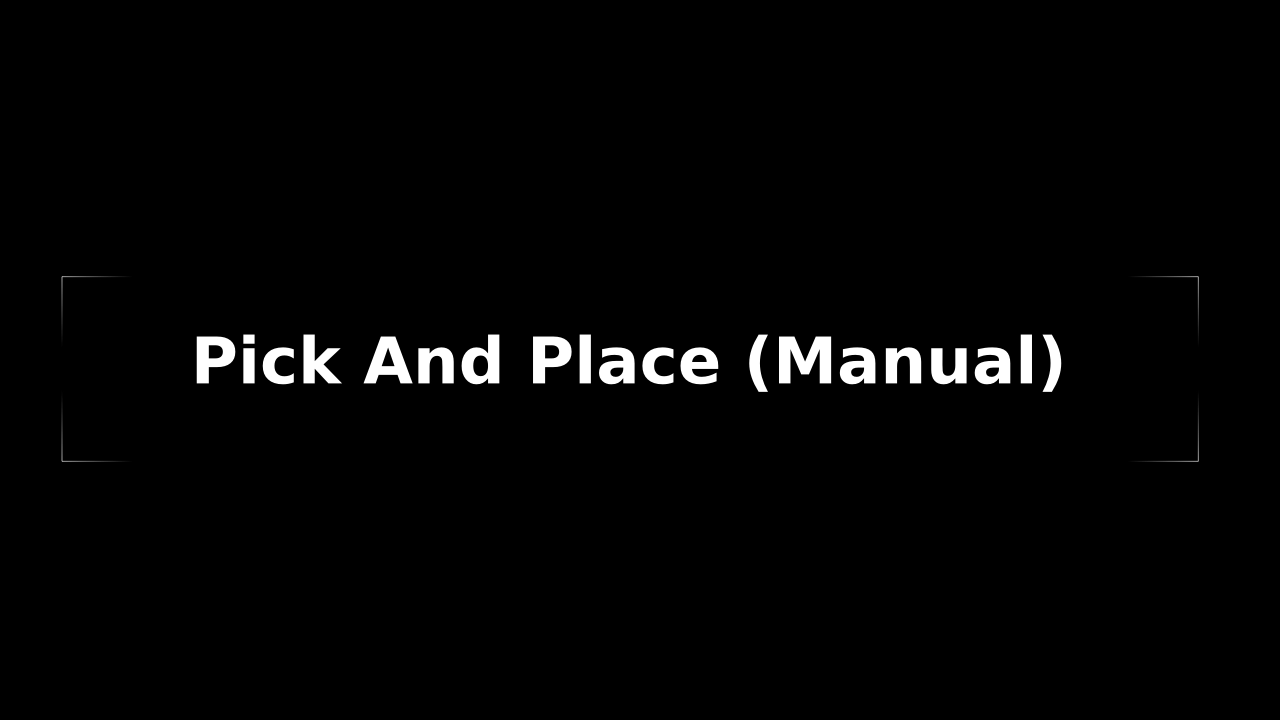
\includegraphics[width=0.6\linewidth]{demo}}{VPlayer.swf}
		\end{center}
	\end{frame}

	\section{References}
	\begin{frame}[allowframebreaks]
		\frametitle{References}
		
		\bibliography{references}
		\bibliographystyle{unsrt}		
	\end{frame}
	
\end{document} 